\section{Experimental analysis}
\label{sec:experimental_analysis}
    \subsection{Task}
      \label{sec:task}
        As mentioned in the introduction, the task consists in classifying sentences
        based on the sentiment expressed by them. The dataset is composed of reviews
        of hotels from the TripAdvisor website, labelled with a score from 1 to 5 stars. \\ 
        
        After the training of the models, the desired output is a class, in the range from 
        1 to 5 stars in the first place, and in the range [0, 2] in the second place, where 
        0 is negative, 1 is neutral and 2 is positive. The second classification task
        is expected to perform better, since it reduces the amount of possible classes
        and the ambiguity of intermediate scores. \\
        
        Furthermore, such task is performed with the purpoose of not only gather 
        metrics about the generalization capabilities of the architectures implemented,
        but also to compare the performance of the two. \\     

    \subsection{Experimental settings}
      \label{sec:experimental_settings}
        All the experiments were run on a machine with a NVIDIA RTX 3060 mobile GPU, 6 GB of VRAM.
        All the validations were performed using $12.7\%$ of the total dataset.


        \subsubsection{LSTM-RNN}
        \label{subsubsec:lstm_rnn}
            In order to determine the best hyperparameters for the LSTM-RNN model, a grid
            search was performed in the space of the hyperparameters, using the f1 score on
            validation set as metric to choose the best configuration. The hyperparameters 
            involved were the learning rate, the dropout rate, the number of hidden units
            and the weight decay. \\ 
            (\textbf{bold} values are the best ones found):

            \begin{table}[H]
                \centering
                \begin{tabular}{l c c c}
                    \toprule
                    \multicolumn{1}{l}{\textbf{Hyperparameter}} & \multicolumn{3}{c}{\textbf{Values}} \\                  \midrule
                    Dropout & 0 & 0.1 & \textbf{0.3} \\
                    Learning rate & 0.001 & 5e-4 & \textbf{1e-4} \\
                    hidden units & 64 & \textbf{128} & 256 \\
                    weight decay & 0 & \textbf{1e-5} & 1e-4 \\
                    \bottomrule
                \end{tabular}
                \label{tab:lstm_hyperparams}
            \end{table}

            It is interesting to note that the f1 score and validation loss of the model
            in the first experiments remained unchanged for the first $25\approx40$ epochs, 
            then the model started to learn. Since such behavior was present without 
            regularization too, and was probably due to the fact that the model is initialized 
            with random weights and the gates of the LSTM were still learning when to open 
            and close, thus leading to a stable high validation loss, immediate consequence 
            of gradient vanishing.\\

            As a solution, in the second iteration the model was modified to make a 
            mean pooling of the hidden states of the LSTM, which are only then passed to
            the classification head. Such change allowed the model to learn from the 
            beginning of the training, leading to better performances.\\

            It should be noted that the patience of early stopping was set to 10 epochs and
            triggers on f1 score. In the first implementation a minimum of 40 epochs to be trained
            was set to avoid the early stopping to stop the training before starting to learn. In the last version
            such threshold was set to 0, since the vanishing problem wasn't present anymore with the same
            relevance.\\ 

            \begin{figure}[H]
              \centering
              \begin{minipage}{0.48\textwidth}
                \centering
                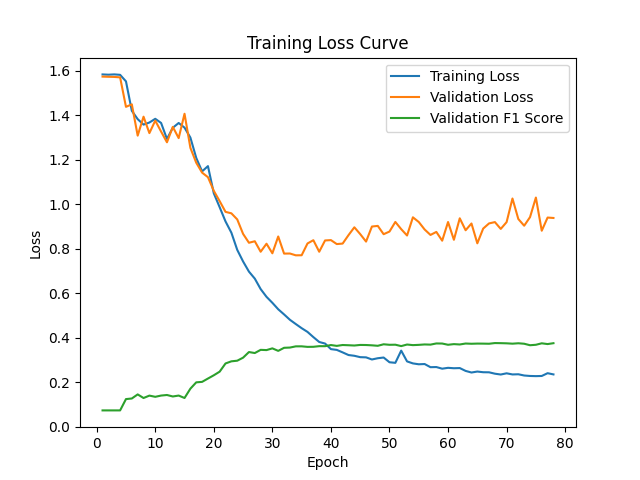
\includegraphics[width=\textwidth]{images/loss_first.png}
                \label{fig:lstm_training_curve_initial}
              \end{minipage}\hfill
              \begin{minipage}{0.48\textwidth}
                \centering
                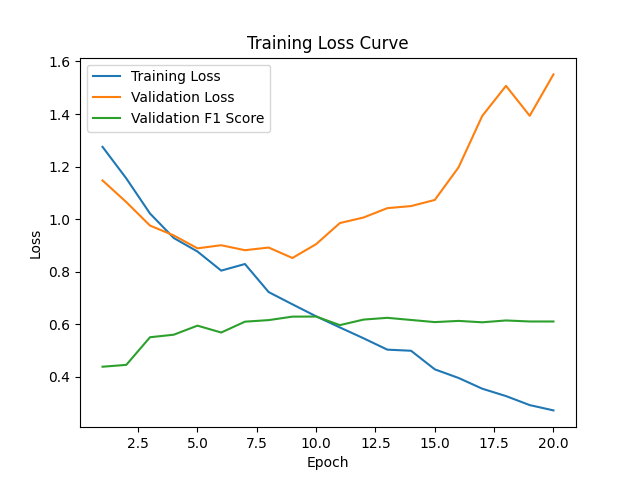
\includegraphics[width=\textwidth]{images/loss_second.png}
                \label{fig:lstm_training_curve_meanpool}
              \end{minipage}
              
                \caption{Training curves in first (left) and second (right) implementation of the LSTM-RNN model.}          
            \end{figure}

            In both cases, the model was trained using the ADAM optimizer, with a batch size of 16,
            exploiting the functions implementend in the torch library to calculare loss and gradients.
            Overall, the training of the model took approximately 90 seconds. \\

        \subsubsection{RoBERTa Transformer}
        \label{subsubsec:roberta}
            The second model implemented is a \texttt{RoBERTaForSequenceClassification} transformer,
            already pretrained, thus the fine-tuning is performed on the dataset adjusting only
            the classification head and a rank-32 LoRA applied to query and value matrices
            of the attention layers. Dropout was set to 0.1, effectively introducing a form
            of control over model complexity. Such design choices allowed to substantially reduce 
            the number of parameters to train:
            \[\text{Trainable parameters:} \quad 2,368,522 / 126,423,562 \approx 1.87\%\]
            Allowing to train the model on a single GPU and perform model selection too.
            The grid search was performed taking into account the loRA dropout, the loRA alpha,
            the learning rate and the weight decay. Here too the validation f1 score was used
            as metric to choose the best hyperparameters. In particular, the hyperparameters 
            chosen for the model were: \\
            (\textbf{bold} values are the best ones found): 

            \begin{table}[H]
                \centering
                \begin{tabular}{l c c c}
                    \toprule
                    \multicolumn{1}{l}{\textbf{Hyperparameter}} & \multicolumn{3}{c}{\textbf{Values}} \\                  \midrule
                    LoRA Dropout & 0 & \textbf{0.1} & 0.3 \\
                    LoRA Alpha & 16 & \textbf{32} & 64 \\
                    Learning rate & 1e-5 & 2e-5 & \textbf{3e-5} \\
                    Weight decay & 0 & \textbf{1e-5} & 1e-4 \\
                    \bottomrule
                \end{tabular}
                \label{tab:roberta_hyperparams}
            \end{table}

            The model was trained using the ADAMW optimizer, with a batch size of 16. Raising such
            value even more might have led to better results, but the GPU VRAM was not enough to
            support it. Thanks to the HuggingFace \texttt{trainer} structure it was possible
            to enable mixed precision training with FP16, thus reducing substantially the memory
            required to train the model effectively. \\

            Differently from the LSTM-RNN model, the RoBERTa model required much less iterations
            to learn, stopping training after only 5 epochs. Nevertheless, each epoch required
            a longer time to be perfomed, of about 6 minutes each, for a total of 28 minutes. \\



    \subsection{Results} 
    \label{sec:results}
        In this section the results of the two models are provided, based on the three 
        main metrics used to evaluate the performance of classification:
        \begin{itemize}
            \item \textbf{Precision}: the ratio of true specific class predictions over the 
                            total number of same specific class predictions made by the model.
            \item \textbf{Recall}: the ratio of true specific class predictions over the total 
                            number of same specific class instances in the dataset.
            \item \textbf{F1 score}: the harmonic mean of precision and recall, which is a good
                            measure of the model's accuracy when dealing with imbalanced datasets,
                            calculated as:
                        \[F1 = 2 \cdot \frac{\text{precision} \cdot \text{recall}}{\text{precision} + \text{recall}}\]
        \end{itemize}

        \subsubsection{LSTM-RNN}
        \label{subsec:lstm_results}
            The confusion matrices of the LSTM-RNN model is shown in the following figure:

            \begin{figure}[H]
              \centering
              \begin{minipage}{0.48\textwidth}
                \centering
                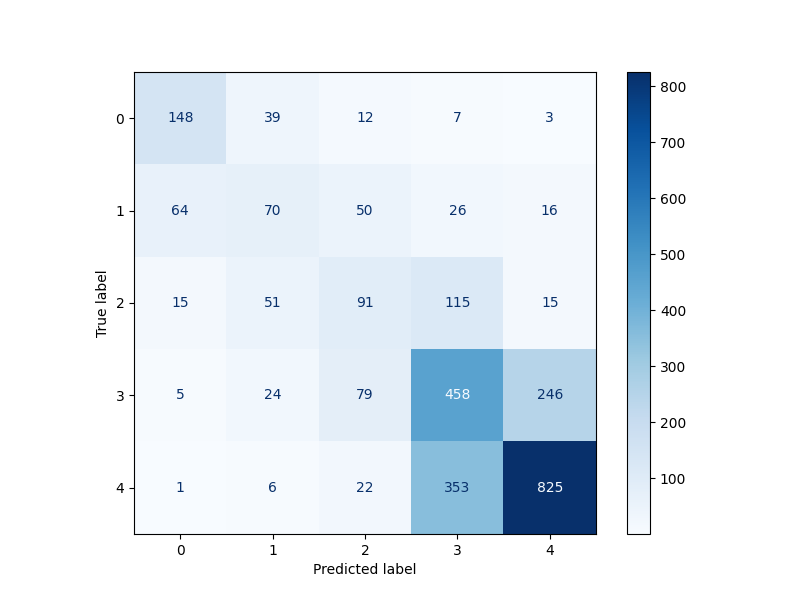
\includegraphics[width=\textwidth]{images/confusion_matrix_lstm.png}
                \caption{5-class confusion matrix, LSTM.}
              \end{minipage}\hfill
              \begin{minipage}{0.48\textwidth}
                \centering
                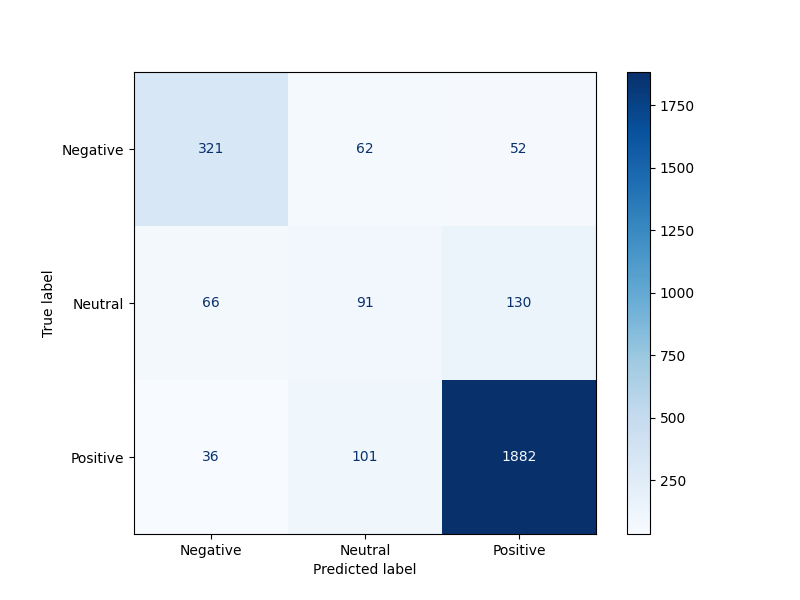
\includegraphics[width=\textwidth]{images/confusion_matrix_lstm_sentiment.png}
                \caption{3-class confusion matrix, LSTM.}
              \end{minipage}  
            \end{figure} 

            from such matrices it is possible to derive the following metrics:

            \begin{table}[H]
                \centering
                \begin{minipage}{0.48\textwidth}
                    \centering
                    \begin{tabular}{l c c c}
                        \toprule
                        \textbf{Class} & \textbf{Precision} & \textbf{Recall} & \textbf{F1} \\                  
                        \midrule
                        1 star & 0.64 & 0.71 & 0.67 \\
                        2 stars & 0.37 & 0.31 & 0.34 \\
                        3 stars & 0.36 & 0.32 & 0.34 \\
                        4 stars & 0.48 & 0.56 & 0.52 \\
                        5 stars & 0.75 & 0.68 & 0.71 \\
                        \midrule
                        weighted avg. & 0.59 & 0.58 & 0.58 \\
                        \bottomrule
                    \end{tabular}
                    \label{tab:5-class_lstm_metrics}
                \end{minipage}\hfill
                \begin{minipage}{0.48\textwidth}
                    \centering
                    \begin{tabular}{l c c c}
                        \toprule
                        \textbf{Class} & \textbf{Precision} & \textbf{Recall} & \textbf{F1} \\                  
                        \midrule
                        Negative & 0.76 & 0.74 & 0.75 \\
                        Neutral & 0.36 & 0.32 & 0.34 \\
                        Positive & 0.91 & 0.93 & 0.92 \\
                        \midrule
                        weighted avg. & 0.83 & 0.84 & 0.83 \\
                        \bottomrule
                    \end{tabular}
                    \label{tab:3-class_lstm_metrics}
                \end{minipage}\hfill
            \end{table}

            It appears that the model is able to classify the reviews quite accurately with
            3 classes, but it struggles with the 5-class classification as the actual discrimination between 4 and 
            5 stars is not very concise, with a lot of 4 stars reviews classified as 5 stars
            and vice versa. Furthermore, the model appears quite confused for all the minority classes,
            which is to be expected given the small proportion of such classes in the dataset. \\

            The overall accuracy of the model is $58\%$ for the 5-class classification, that still
            is a good result given the small dataset and the well known difficulty of RNN to learn
            over quite long sequences. The accuracy for the 3-class classification is $84\%$,
            and in contrast to the $33\%$ of a random classifier, it holds quite well, given the
            minimal amount of training required. \\

        \subsubsection{RoBERTa Transformer}
        \label{subsec:roberta_results}
            The confusion matrices of the RoBERTa model is shown in the following figure:

            \begin{figure}[H]
              \centering
              \begin{minipage}{0.48\textwidth}
                \centering
                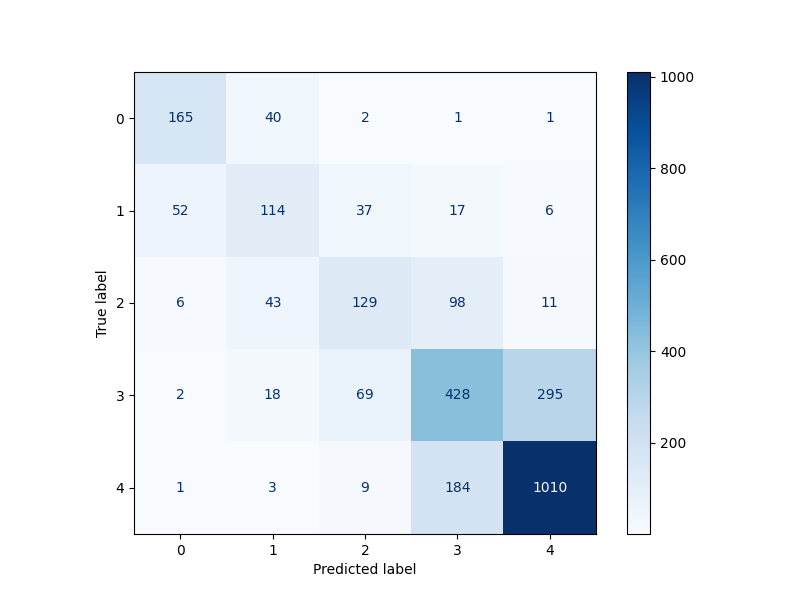
\includegraphics[width=\textwidth]{images/confusion_matrix_transformer.png}
                \caption{5-class confusion matrix, RoBERTa.}
              \end{minipage}\hfill
              \begin{minipage}{0.48\textwidth}
                \centering
                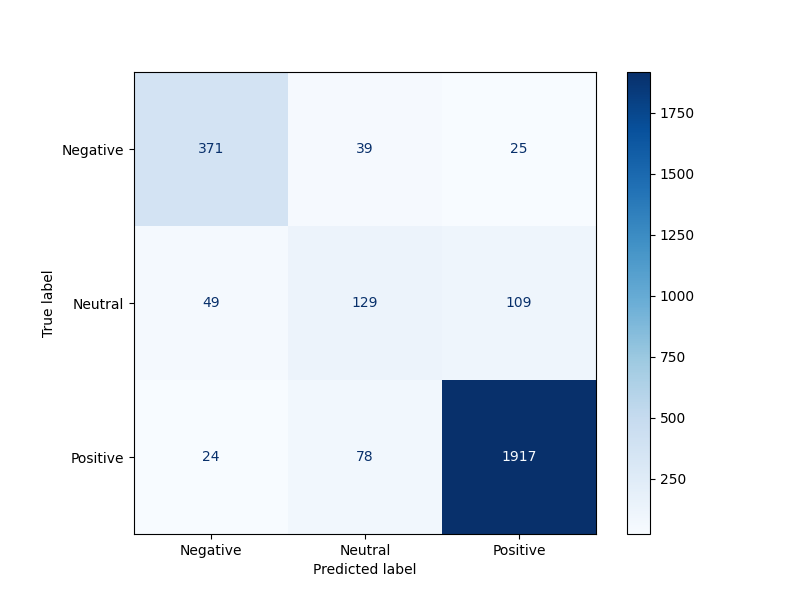
\includegraphics[width=\textwidth]{images/confusion_matrix_transformer_sentiment.png}
                \caption{3-class confusion matrix, RoBERTa.}
              \end{minipage}  
            \end{figure}

            that bring to the following metrics:

            \begin{table}[H]
                \centering
                \begin{minipage}{0.48\textwidth}
                    \centering
                    \begin{tabular}{l c c c}
                        \toprule
                        \textbf{Class} & \textbf{Precision} & \textbf{Recall} & \textbf{F1} \\                  
                        \midrule
                        1 star & 0.73 & 0.79 & 0.76 \\
                        2 stars & 0.52 & 0.50 & 0.51 \\
                        3 stars & 0.52 & 0.45 & 0.48 \\
                        4 stars & 0.59 & 0.53 & 0.56 \\
                        5 stars & 0.76 & 0.84 & 0.80 \\
                        \midrule
                        weighted avg. & 0.66 & 0.67 & 0.67 \\
                        \bottomrule
                    \end{tabular}
                    \label{tab:5-class_roberta_metrics}
                \end{minipage}\hfill
                \begin{minipage}{0.48\textwidth}
                    \centering
                    \begin{tabular}{l c c c}
                        \toprule
                        \textbf{Class} & \textbf{Precision} & \textbf{Recall} & \textbf{F1} \\                  
                        \midrule
                        Negative & 0.84 & 0.85 & 0.84 \\
                        Neutral & 0.52 & 0.45 & 0.48 \\
                        Positive & 0.93 & 0.95 & 0.94 \\
                        \midrule
                        weighted avg. & 0.88 & 0.88 & 0.88 \\
                        \bottomrule
                    \end{tabular}
                    \label{tab:3-class_roberta_metrics}
                \end{minipage}\hfill
            \end{table}

            The results of the RoBERTa model appear to be better than the LSTM-RNN model, 
            and the level of generalization the model achieved is quite good, with an 
            acceptable classification capability for minority classes too. The addition of 
            attention mechanisms and the pretraining yield better long distance information
            dependecies.\\
            
            Such additional features bring accuracies of $67\%$ and $88\%$ for the 5-class 
            and 3-class, with improvements of $15.5\%$ and $4.8\%$ respectively. The great 
            improvement in 5-star classification is a demonstrarion of the superior context
            understanding of the transformer architecture, which is able to capture finer
            differences in the reviews. \\

        \subsection{Comparison with Literature}
        \label{subsec:comparison_literature}
            As term of comparison, the results of the presented model will be 
            compared with the results of the paper \textit{"Sentiment Analysis of 
            Hotel Reviews With LSTM And ELECTRA"} by \cite{husein2023sentiment}, 
            which presents a 3-class sentiment analysis on scraped hotel reviews.
            The models used in the paper are an LSTM and a discriminator encoder
            called ELECTRA.\\

            To make a fair comparison, some further training instances will be done to the 
            presentented models with an oversampled and an undersampled version
            of the dataset used in this project, since the \citet{husein2023sentiment}'s
            one is undersampled too to equalize the amount of entries for each class. For 
            this purpose, the oversampled dataset will have all the classes as numerous as 
            the 5-star reviews, that amount to $8270$, and the undersampled done will have 
            all classes as popolated as the 1-star class, that has dimension $1236$.\\

            \begin{table}[H]
                \centering
                \begin{tabular}{l c c c c}
                    \toprule
                    \textbf{Model} & \textbf{Accuracy} & \textbf{Precision} & \textbf{Recall} & \textbf{F1} \\                  
                    \midrule 
                    LSTM - US & 0.73 & 0.74 & 0.73 & 0.73 \\
                    LSTM & 0.84 & 0.83 & 0.84 & 0.83\\
                    LSTM - OS & 0.82 & 0.84 & 0.82 & 0.83 \\
                    RoBERTa - US & 0.80 & 0.79 & 0.80 & 0.79 \\
                    RoBERTa & 0.88 & 0.88 & 0.88 & 0.88 \\
                    RoBERTa - OS & 0.86 & 0.86 & 0.86 & 0.86 \\
                    ELECTRA \cite{husein2023sentiment} & 0.47 & 0.33-0.56 & 0.38-0.62 & 0.35-0.59 \\
                    LSTM \cite{husein2023sentiment} & 0.30 & 0.38-0.40 & 0.29-0.50 & 0.28-33 \\
                    \bottomrule
                \end{tabular}
                \label{tab:comparison_literature}
            \end{table}

            The results shows that on the native dataset transformers work better than RNNs,
            capable of capturing finer differences in the reviews, but within over-sampling
            the LSTM-RNN results to be comparable to the RoBERTa based model. Such behavior
            hints that LSTM based architectures are better suited for learning from 
            balanced datasets. On the other side, the RoBERTa implementation suffers from
            ripetitive data, which leads to a worse performance, probably due to 
            overfitting.\\

            Furthermore, the undersampled versions show that, even if the trasformer based
            implementation is able to generalize better than ELECTRA \citep{husein2023sentiment},
            it definitely suffers from the lack of data, leading to a worse performance. Nevertheless,
            both models are able to outperform the LSTM based and ELECTRA model introduced 
            by \citet{husein2023sentiment}.